\section{Overview of inventory generation methods in literature}




    \paragraph{Plant Data}Energy usage and mass flows are  measured in an existing chemical plant in industrial scale. This data is considered the most precise among the other inventory generation methods. Errors in measure procedure and regional differences may decrease data quality. 
    
    
%    why?:\\
%minor simplifications, assumptions\\
%aiming for realistic inventory\\

%how?\\
%measuring values on site of chemical plant to compile inventory: mass flows(educts, products, wastes, emissions, catalyst usage, auxiliary material, T, p, utility usage, composition)representation of industrial Measuring values on site of chemical plants to compile
    \paragraph{Process Simulation}Chemical process simulation software is used to extract inventory information. In order to perform the simulation, much data is needed. This data consists among others of process flow sheet and sizes of equipment as well as thermodynamic values through all unit operations. Obtaining this data occupies much time. Additionally a high level of knowledge and experience with the software tool is necessary to perform the simulation. Because of this disadvantages this method is not ideal for establishing life cycle data bases fastly and thus this work will not further analyse this method.
    \paragraph{Process Calculation}inventory is derivered from detailed process design equations. Empirical or thermodynamical equations for the energy usage of chemical processes like pumping, heating, reaction, destillation. 
    \paragraph{Process Scale-Up} (need reference: there is this scale-up paper about equipment sizes) Measured data obtained in laboratory is extrapolated to industrial plant scale. Gathering the input data requires much time (beleg!) and reliability of scale up???  makes this method not usable for establishing LCA databases.
    \paragraph{Stoichiometry}balaced stoichiometric equation provides mass flows of reactants and products. In more detailed versions of this method information about the energy usage can be obtained by basis thermodynamic considerations.
    \paragraph{Ecoinvent approach 'Gendorf'}Massflows are generated analoguous to the stoichiometric approach. Direct emissions of reactants are estimated by a rule of thumb. The energy requirement is replaced by an medial value for the production of chemicals obtained from the chemical plant in Gendorf, Germany. 
    \paragraph{Molecular Structure Models} Statistical methods that find correlation between chemical properties and environmental impact indicators. Usually they directly output a Life Cycle Impact values, skipping the Life Cycle Inventory Analysis\cite{pavatker.2017}.
    \paragraph{Proxies}If there is enough expert knowledge, one chemical can represent another one as proxy. To decide on suitable proxies deep knowledge on synthesis chemistry is necassary \cite{pavatker.2017}.

    \paragraph{Omitting} If there is no data available at all about the process, all mass flows in the inventory of the process except the desired output stream have to be left out. This is called the omitting.  Other Reasons for doing so are the presence of complex structures or mixtures of substances as well as unknown quantities of used chemicals \cite{2019.Pavatker}.
    
\subsection{Process Calculation}
 
 (for everything \cite{pavatker.2017})
detailed calculations of subprocesses. Depending level of detail it can cover the energy requirements of the reactor including stirring, the separation process, pumps and a dryer. Additionally Process Calculation usually uses a method to quantify fugitive emissions occurring during the process.


assumptions: yield, solvent recovery and educt recycling: quantification of mass flows of substances

basis: energy and mass balances for estimation of inventory plus empirical design equations

static values no f of time, temp, p

data sources: process description (patents, scientific literature): all names of substances

advanced: build on basis: additional scale, equipment efficiency, heat transfer operations, heat integration, reflux, reactor geometry

equations (Pavatker cites: see note paper)


advantages:

able to include all unit processes

detailed model of process supposed to produce realistic inventory

disadvantages:

much knowledge process design engineering needed
detailed equipment data necessary: Example: \cite{Piccino.2017} Detailed analysis of the energy requirement of a reactor also considers heat losses. In order to calculate heat losses the insulation thickness and heat conductance is to be known. It is hard to obtain such equipment specific data in an automated way, for the purpose of generating Life Cycle Assessment databases.

many data from process description need manual processing: limiting automatic inventory generation for databases

\begin{figure}[htp]
        \centering
        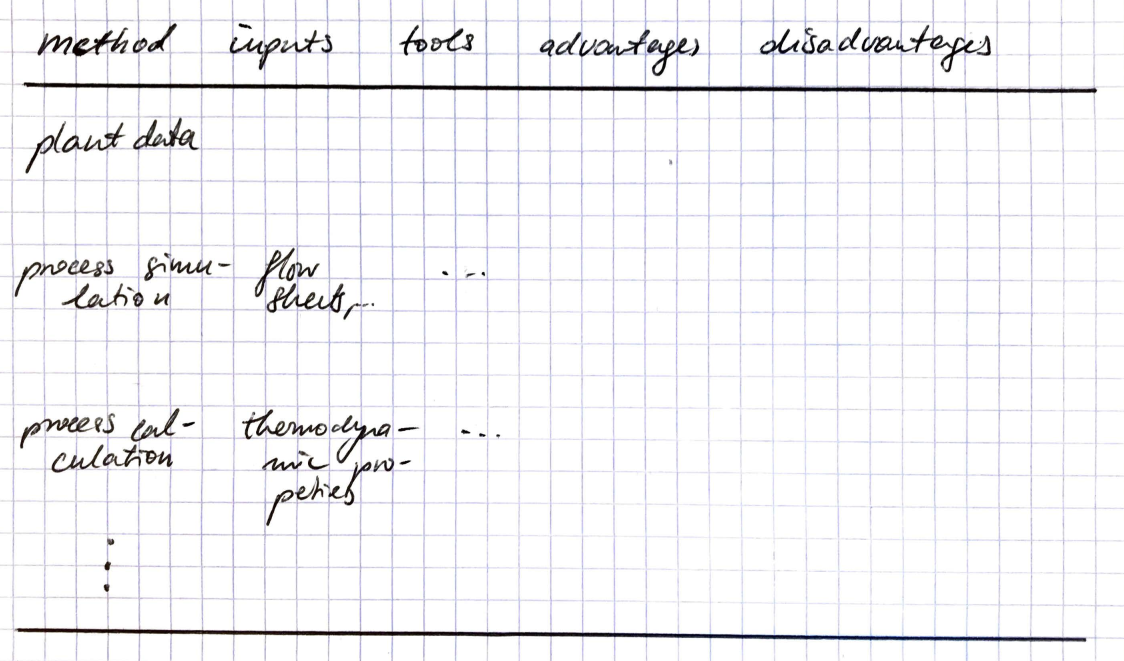
\includegraphics[width=0.9\textwidth]{images/advantages.PNG}
        \caption{Evaluation of methods}
        \label{fig:evaluation}
\end{figure}


overview table: hierarchy,level of detail, time, resources,  process based, statistical , , , automatable\\

\begin{table}[]
    \centering
    \begin{tabular}{c|c|c}
-                           & class             & automatable for databases\\
Plant Data                  & process based     & ?\\
Process Simulation          &  process based    & no\\
Process Calculation         &  process based    & yes\\
Process Scale-Up            & process based     & no\\
Stoichiometry               & process based     & yes\\
Molecular Structure Models  & statistical based & yes\\
Proxies                     &  process based    & no\\
Omitting                    &   -               & yes\\
    \end{tabular}
    \caption{Overview inventory generation methods}
    \label{tab:my_label}
\end{table}

explain in list: process based, \\

explain in list: model process, process based\\

explain in list: level of detail, hierarchy\\

examine in each subsection: assumptions, simplifications and considerations and if  automatable, suitable for databases in each following subsection\\

focus this work: automatable, suitable for databases, fast, cheap, process based, they will be applyed in case study later

\cite{pavatker.2019} distinguishes three levels of stoichiometry (see Table \ref{3levelsstoichiometry}): explaine table 

\begin{table}[]
    \centering
    \begin{tabular}{c c c}
    level   & required data                         & calculation\\
     1      & balances reaction + molecular weights & mass balance \\
     2      & balanced reaction + heat of reaction + heat capacity + molecular weights & mass \& energy balance\\
     3      & level 2 or level 1 + yield & mass \& energy balance\\
    \end{tabular}
    \caption{required data and calculation in threee levels of stoichiometry method}
    \label{3levelsstoichiometry}
\end{table}{}